% replace all text with your own text.
% in this template few examples are mention
\chapter{Methodology}
\label{ch:method} % Label for method chapter
\section{Dataset Description and Data Exploration}
The diabetes data set is originated from kaggle \citep{dataset}. The dataset contains 2000 patients and their corresponding 9 unique attributes. The nine attributes that are used for the prediction of diabetes are `Pregnancies`, 
`Glucose`, `BloodPressure`, `SkinThickness`, `Insulin`, `BMI`, `DiabetesPedigreeFunction`, `Age`, `Outcome`. The `Outcome` attribute is taken as a dependent or target variable, and the remaining eight attributes are taken as independent feature variables. The diabetes attribute `Outcome` consists of binary value where 0 means non-diabetes, and 1 implies diabetes.

\begin{figure}[ht]
    \centering    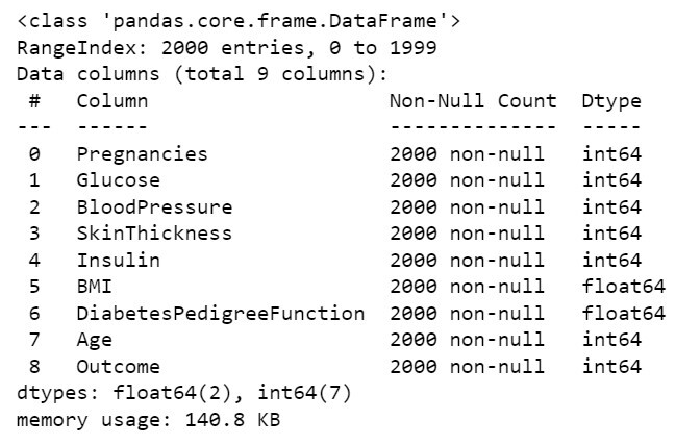
\includegraphics[scale=1.0]{figures/data_info.pdf}
    \caption{Dataset attributes and their data types.}
    \label{fig:capture_a}
\end{figure}
Here, all the attributes in Fig~\ref{fig:capture_a} are numeric and there are no null values. 
\begin{figure}[ht]
    \centering    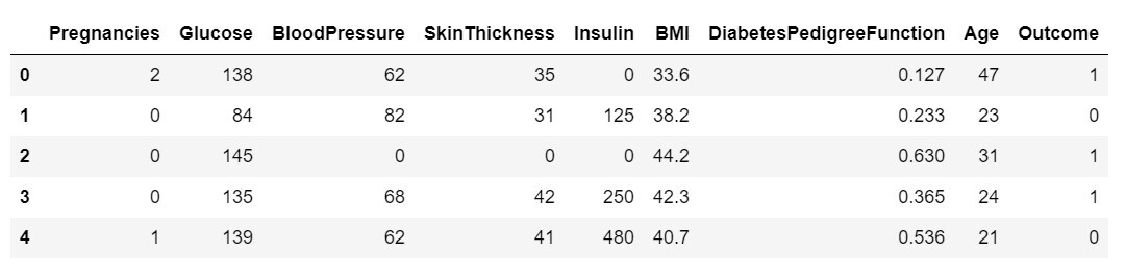
\includegraphics[scale=0.8]{figures/data_top5.pdf}
    \caption{Top 5 patients data.}
    \label{fig:capture_b}
\end{figure}

\subsection{Correlation Matrix}
\label{subsec:corr_matrix}
A correlation matrix is a powerful tool for data analysis. It is a statistical technique used to evaluate the relationship between two variables in a dataset. It provides a correlation coefficient for each cell. The correlation coefficient value remains in the range between -1 and 1.

The correlation coefficient value -1 indicates notable negative linear correlation. The coefficient value 1 indicates notable positive linear correlation. The coefficient value 0 indicates no linear correlation.

A correlation matrix helps summarize data, identify patterns, and make decisions based on relationships between attributes. It helps us to gain insights for building better machine learning models by understanding which attributes are correlated.

\begin{figure}[ht]
    \centering    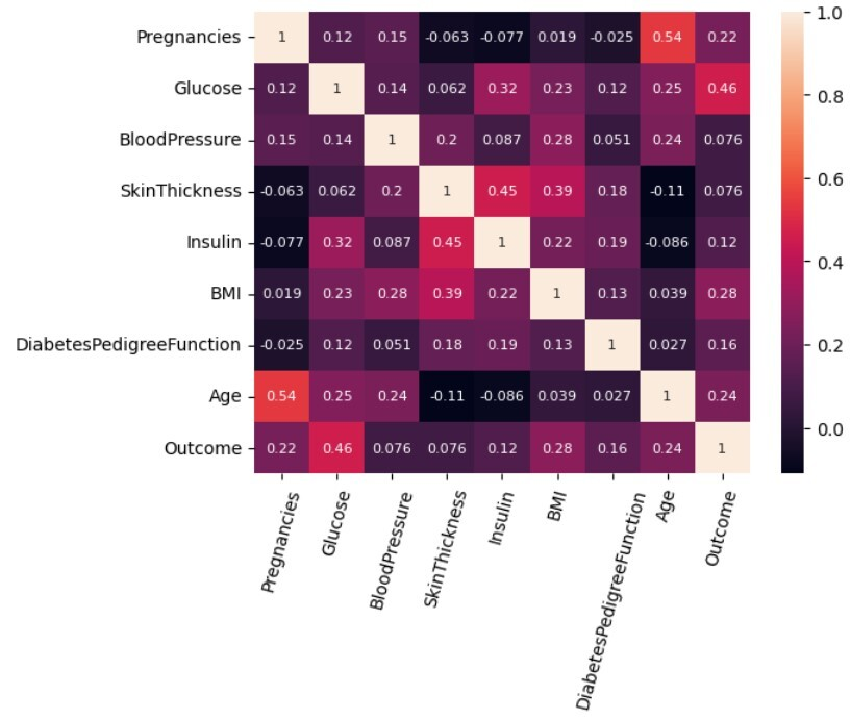
\includegraphics[scale=0.8]{figures/data_correlation.pdf}
    \caption{Correlation Matrix}
    \label{fig:capture_c}
\end{figure}

\subsection{Data Distribution using Histograms}
Fig~\ref{fig:capture_d} gives a better feel than the raw numbers and percentiles of the distributions of our numerical attributes. It shows how each feature and label is distributed along different ranges which further confirms the need for scaling. Next, wherever you see discrete bars, it basically means that each of these is actually a categorical variable. We will need to handle these categorical variables before applying Machine Learning. Our outcome labels have two classes, 0 for no disease and 1 for disease. 
\begin{figure}[ht]
    \centering    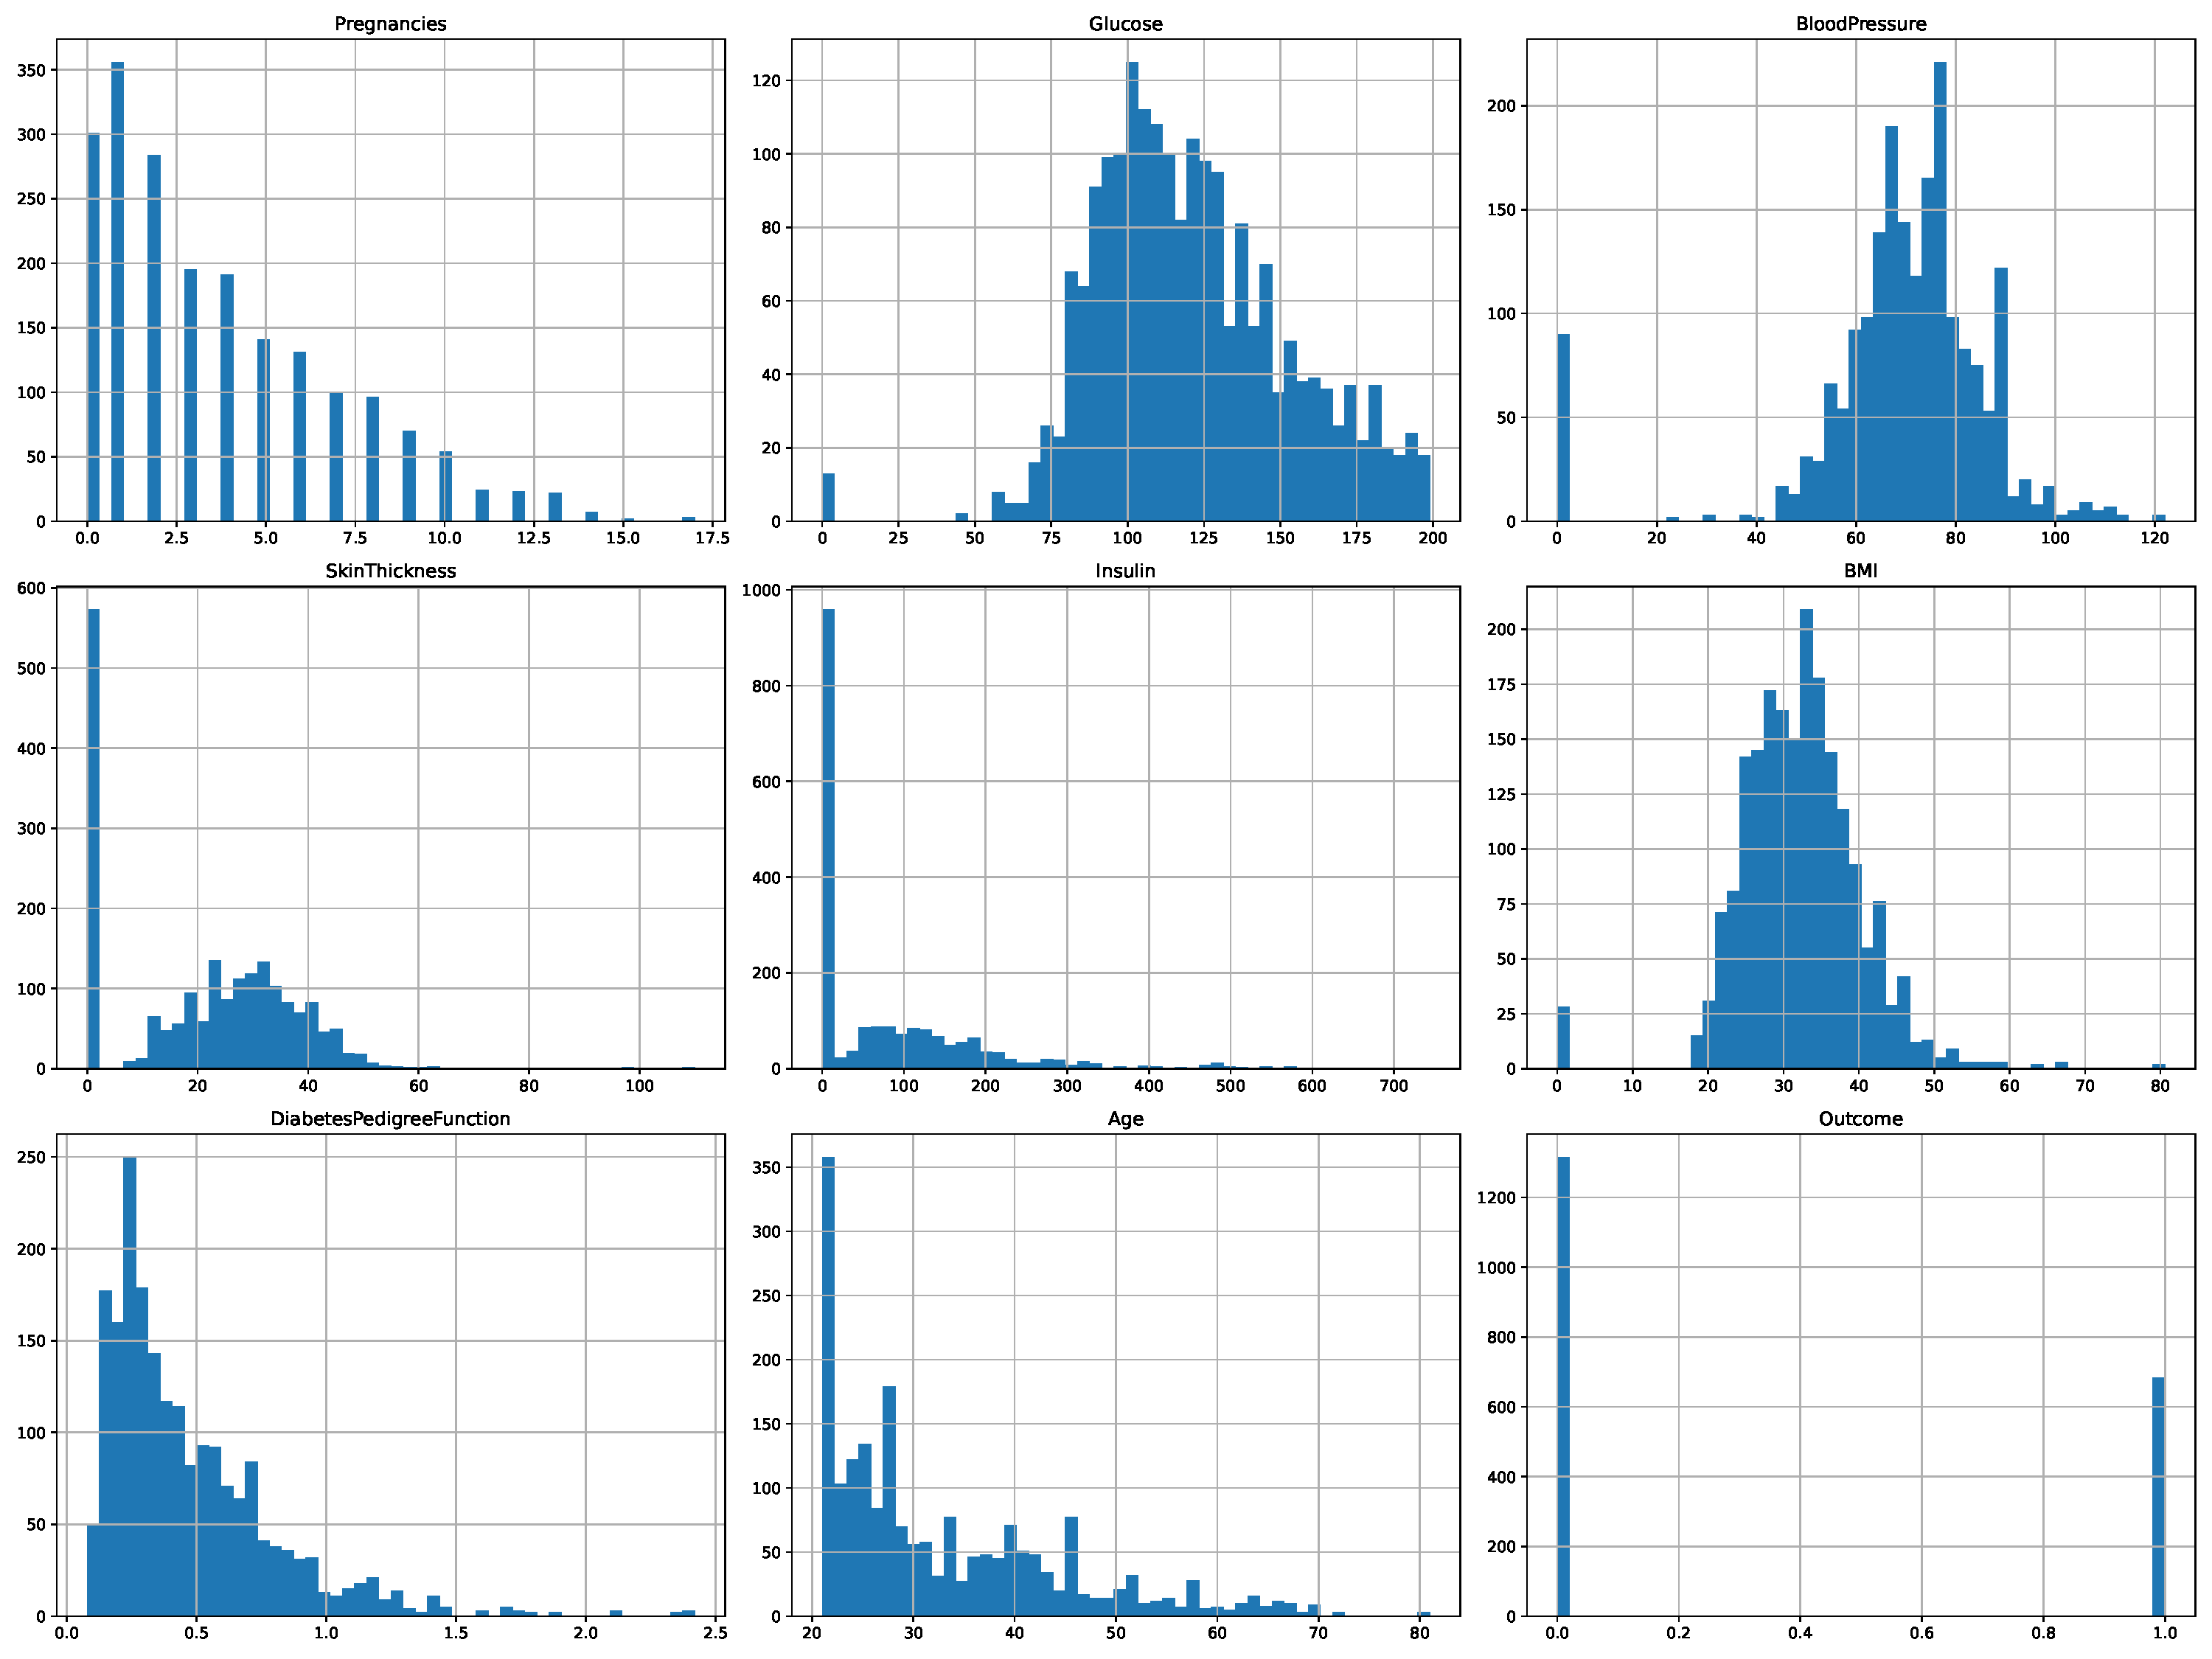
\includegraphics[scale=0.8]{figures/data_attr_distribution.pdf}
    \caption{Data Distribution for each attribute}
    \label{fig:capture_d}
\end{figure}

\subsection{Bar plot for Outcome class}
Fig~\ref{fig:capture_e} shows that the data is biased towards data points having outcome value as 0 which means that diabetes was not present actually. The number of non-diabetics is almost twice the number of diabetic patients.

Out of the 2000 instances, 1316 are associated with non-diabetic patients, while the remaining 684 pertain to diabetic patients.
\begin{figure}[ht]
    \centering    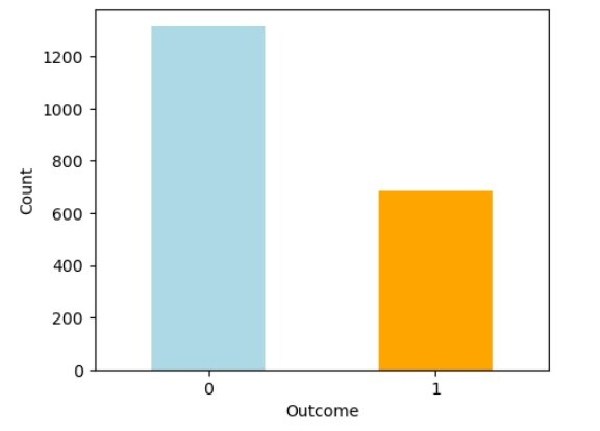
\includegraphics[scale=0.8]{figures/data_distribution.pdf}
    \caption{Distribution of Outcome (0s and 1s)}
    \label{fig:capture_e}
\end{figure}


\section{Data Preprocessing}

Data preprocessing helps to transform data used to built a model which gives higher performance metrics. This process performs various functions like handling missing values, normalization and feature selection to improve the quality of data.

\subsection{Missing Values Identification}
Fig~\ref{fig:capture_a} indicates the absence of null values for all attributes. However, Fig~\ref{fig:capture_b} illustrates instances of zero values for attributes which are irrelevant and need to handled. Table~\ref{tab:table-01-missing-values} shows the number of zero values for each attribute.

 \begin{table}[ht!]
    \centering
    \caption{The number of zero missing values in dataset}
    \begin{tabular}{lrrrrr}
Attributes & No.of missing values (Zero) \\
Pregnancies & 301 \\
Glucose & 13 \\
BloodPressure & 90 \\
SkinThickness & 573 \\
Insulin & 956 \\
BMI & 28 \\
DiabetesPedigreeFunction & 0 \\
Age & 0 \\
\end{tabular}


    \label{tab:table-01-missing-values}
\end{table}

Here, we have observed numerous attributes with zero values, impacting the data quality. We replaced the zero values with the corresponding mean values using simpleimputer.

Fig~\ref{fig:capture_b} and Fig~\ref{fig:capture_f} shows the top five patients data. If you compare these figures, Fig~\ref{fig:capture_f} indicates that zero values in Fig~\ref{fig:capture_b} was replaced with mean for each attribute. Now, there are no missing values either null or zero values in each attribute.

\begin{figure}[ht]
    \centering    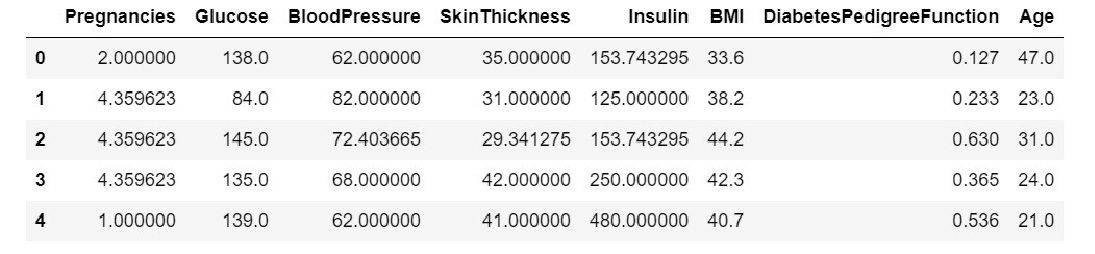
\includegraphics[scale=0.8]{figures/data_info_after_imputer.pdf}
    \caption{Top 5 patients data after handling missing values}
    \label{fig:capture_f}
\end{figure}

\subsection{Feature Selection based on Correlation Coefficient}
After handling missing values, the correlation coefficient is calculated in this method which correlates with the output and input attributes. This was discussed under section~\ref{subsec:corr_matrix}. We have created a Table~\ref{tab:table-02-corr_matrix} to show correlation coefficient values of each attribute towards target attribute.

 \begin{table}[ht!]
    \centering
    \caption{The correlation coefficient values}
    \begin{tabular}{lrr}
 & Correlation Coefficient & Correlation Coefficient after imputation \\
Pregnancies & 0.224437 & 0.249883 \\
Glucose & 0.458421 & 0.488020 \\
BloodPressure & 0.075958 & 0.174481 \\
SkinThickness & 0.076040 & 0.205527 \\
Insulin & 0.120924 & 0.207696 \\
BMI & 0.276726 & 0.282182 \\
DiabetesPedigreeFunction & 0.155459 & 0.155459 \\
Age & 0.236509 & 0.236509 \\
\end{tabular}

    \label{tab:table-02-corr_matrix}
\end{table}

We used 0.2 as a cut-off for relevant attributes. Hence   `BloodPressure` and `DiabetesPedigreeFunction` features are removed. `Pregnancies`, `Glucose`, `SkinThickness`, `Insulin`, `BMI`, and `Age` are our most relevant six input attributes.

\section{Example of a Figure in \LaTeX}
Figure~\ref{fig:chart_a} is an example of a figure in \LaTeX. For more details, check the link:

\href{https://en.wikibooks.org/wiki/LaTeX/Floats,_Figures_and_Captions}{wikibooks.org/wiki/LaTeX/Floats,\_Figures\_and\_Captions}.

\noindent
Keep your artwork (graphics, figures, illustrations) clean and readable. At least 300dpi is a good resolution of a PNG format artwork. However, an SVG format artwork saved as a PDF will produce the best quality graphics. There are numerous tools out there that can produce vector graphics and let you save that as an SVG file and/or as a PDF file. One example of such a tool is the ``Flow algorithm software''. Here is the link for that: \href{http://www.flowgorithm.org/download/}{flowgorithm.org}.
\begin{figure}[ht]
    \centering
    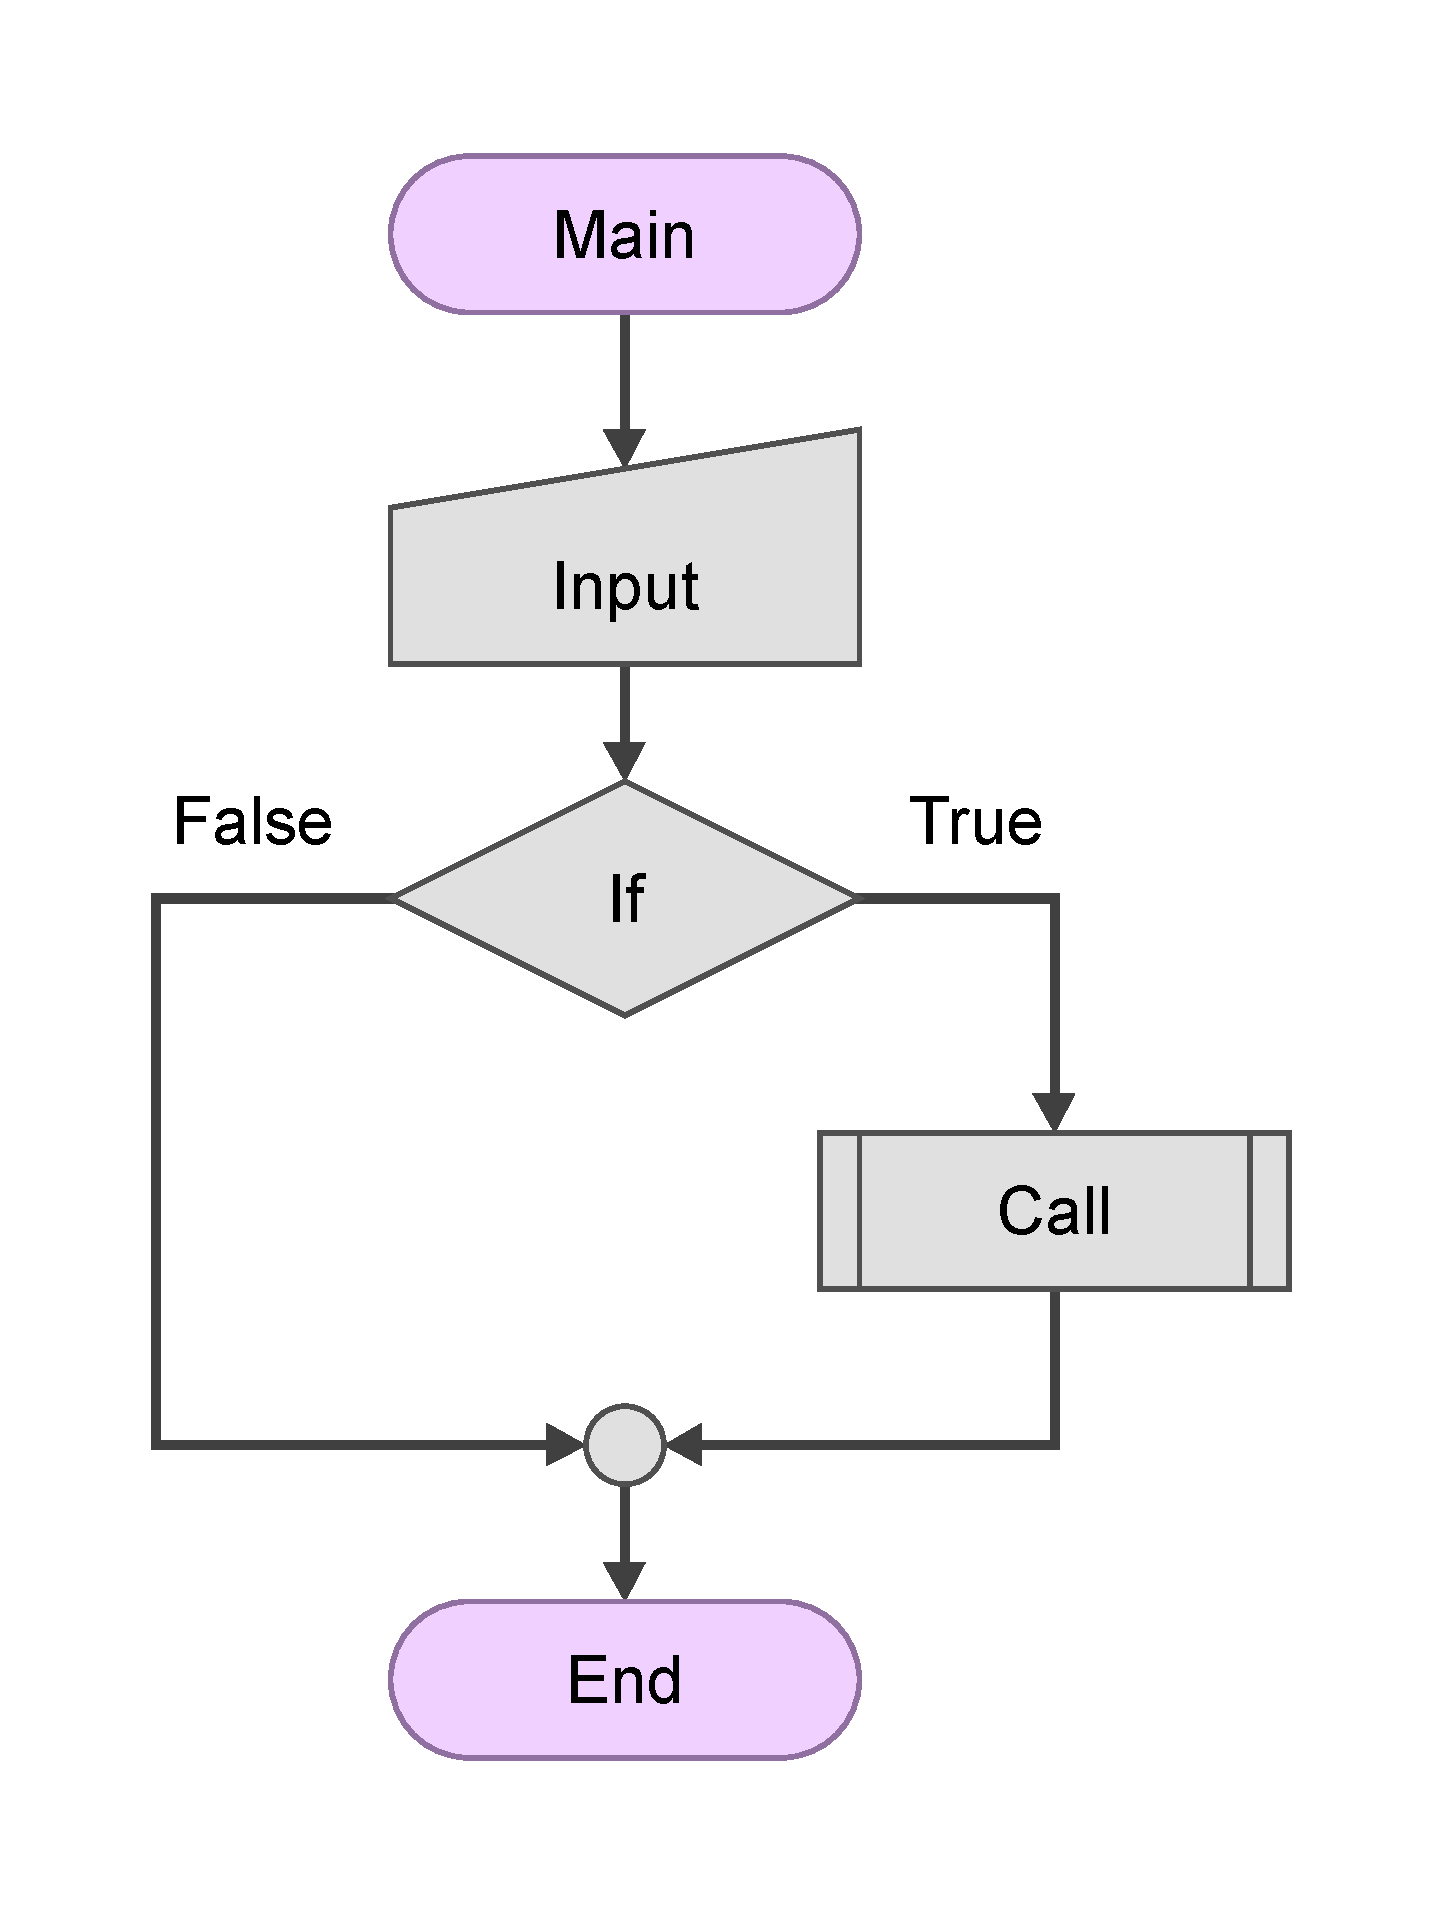
\includegraphics[scale=0.3]{figures/chart.pdf}
    \caption{Example figure in \LaTeX.}
    \label{fig:chart_a}
\end{figure}

\clearpage %  use command \clearpage when you want section or text to appear in the next page.

\section{Example of an algorithm in \LaTeX}
Algorithm~\ref{algo:algo_example} is a good example of an algorithm in \LaTeX.  
\begin{algorithm}
    \caption{Example caption: sum of all even numbers}
    \label{algo:algo_example}
    \begin{algorithmic}[1]
        \Require{$ \mathbf{x}  = x_1, x_2, \ldots, x_N$}
        \Ensure{$EvenSum$ (Sum of even numbers in $ \mathbf{x} $)}
        \Statex
        \Function{EvenSummation}{$\mathbf{x}$}
        \State {$EvenSum$ $\gets$ {$0$}}
        \State {$N$ $\gets$ {$length(\mathbf{x})$}}
        \For{$i \gets 1$ to $N$}                    
        \If{$ x_i\mod 2 == 0$}  \Comment check if a number is even?
        \State {$EvenSum$ $\gets$ {$EvenSum + x_i$}}
        \EndIf
        \EndFor
        \State \Return {$EvenSum$}
        \EndFunction
    \end{algorithmic}
\end{algorithm}
 
\section{Example of code snippet  in \LaTeX}

Code Listing~\ref{list:python_code_ex} is a good example of including a code snippet in a report. While using code snippets, take care of the following:
\begin{itemize}
    \item do not paste your entire code (implementation) or everything you have coded. Add code snippets only. 
    \item The algorithm shown in Algorithm~\ref{algo:algo_example} is usually preferred over code snippets in a technical/scientific report. 
    \item Make sure the entire code snippet or algorithm stays on a single page and does not overflow to another page(s).  
\end{itemize}

Here are three examples of code snippets for three different languages (Python, Java, and CPP) illustrated in Listings~\ref{list:python_code_ex}, \ref{list:java_code_ex}, and \ref{list:cpp_code_ex} respectively.  

\begin{lstlisting}[language=Python, caption={Code snippet in \LaTeX ~and  this is a Python code example}, label=list:python_code_ex]
import numpy as np

x  = [0, 1, 2, 3, 4, 5] # assign values to an array
evenSum = evenSummation(x) # call a function

def evenSummation(x):
    evenSum = 0
    n = len(x)
    for i in range(n):
        if np.mod(x[i],2) == 0: # check if a number is even?
            evenSum = evenSum + x[i]
    return evenSum
\end{lstlisting}

Here we used  the ``\textbackslash clearpage'' command and forced-out the second listing example onto the next page. 
\clearpage  %
\begin{lstlisting}[language=Java, caption={Code snippet in \LaTeX ~and  this is a Java code example}, label=list:java_code_ex]
public class EvenSum{ 
    public static int evenSummation(int[] x){
        int evenSum = 0;
        int n = x.length;
        for(int i = 0; i < n; i++){
            if(x[i]%2 == 0){ // check if a number is even?
                evenSum = evenSum + x[i];
            }
        }
        return evenSum;     
    }
    public static void main(String[] args){ 
        int[] x  = {0, 1, 2, 3, 4, 5}; // assign values to an array
        int evenSum = evenSummation(x);
        System.out.println(evenSum);
    } 
} 
\end{lstlisting}


\begin{lstlisting}[language=C, caption={Code snippet in \LaTeX ~and  this is a C/C++ code example}, label=list:cpp_code_ex]
int evenSummation(int x[]){
    int evenSum = 0;
    int n = sizeof(x);
    for(int i = 0; i < n; i++){
        if(x[i]%2 == 0){ // check if a number is even?
            evenSum = evenSum + x[i];
    	}
    }
    return evenSum;     
}

int main(){
    int x[]  = {0, 1, 2, 3, 4, 5}; // assign values to an array
    int evenSum = evenSummation(x);
    cout<<evenSum;
    return 0;
}
\end{lstlisting}



\section{Example of in-text citation style}
\subsection{Example of the equations and illustrations placement and reference in the text}
Make sure whenever you refer to the equations, tables, figures, algorithms,  and listings for the first time, they also appear (placed) somewhere on the same page or in the following page(s). Always make sure to refer to the equations, tables and figures used in the report. Do not leave them without an \textbf{in-text citation}. You can refer to equations, tables and figures more them once.

\subsection{Example of the equations and illustrations style}
Write \textbf{Eq.} with an uppercase ``Eq`` for an equation before using an equation number with (\textbackslash eqref\{.\}). Use ``Table'' to refer to a table, ``Figure'' to refer to a figure, ``Algorithm'' to refer to an algorithm and ``Listing'' to refer to listings (code snippets). Note that, we do not use the articles ``a,'' ``an,'' and ``the'' before the words Eq., Figure, Table, and Listing, but you may use an article for referring the words figure, table, etc. in general.

 
 

\section{Summary}
Write a summary of this chapter.

~\\[5em]
\noindent
{\huge\textbf{Note:}} In the case of \textbf{software engineering} project a Chapter ``\textbf{Testing and Validation}'' should precede the ``Results'' chapter. See for report organization of such project. 

